%\documentclass[10pt]{beamer}
\documentclass[10pt,handout]{beamer}
\usepackage[english]{babel}
% % \usepackage[backend=biber, style=authoryear-icomp]{biblatex}
\resetcounteronoverlays{exx}
\usepackage{mdframed}
\usepackage{tikz}
\usepackage{blindtext}
\usepackage{tipa}
% \usepackage{cgloss4e}
% \usepackage{gb4e}
% \usepackage{qtree}
\usepackage{cancel}
\usepackage{wrapfig}
\usepackage{soul}
\usepackage{enumerate}
\usepackage{longtable}
\graphicspath{ {.} } % declaramos donde estan las imagenes
\usepackage[labelformat=simple]{subcaption} % para varias imagenes juntas
\renewcommand\thesubfigure{(\alph{subfigure})}
\usepackage[utf8]{inputenc}
\usepackage{amsmath}
\usepackage{amsfonts} % simbolos como el I de matriz identidad
\usepackage{bm}
\usepackage{graphicx} % paquete para ver imagenes
\usepackage{setspace}
\usepackage[T1]{fontenc}
\usepackage{parskip}
\usepackage{color}
\usepackage{framed}
\usetheme{Copenhagen}
\definecolor{frenchblue}{rgb}{0.0, 0.45, 0.73} % ESTE!!!!
\definecolor{myblue1}{RGB}{35,119,189}
\definecolor{myblue2}{RGB}{95,179,238}
\definecolor{myblue3}{RGB}{129,168,207}
\definecolor{myblue4}{RGB}{26,89,142}

\setbeamercolor{block body}{bg=frenchblue!50}
\setbeamercolor*{structure}{fg=frenchblue,bg=blue}
\setbeamertemplate{frametitle}[default][center]
\setlength{\parskip}{12pt}
\useoutertheme{infolines} % me comia mucho espacio de la otra fgorma
\makeatother
\setbeamertemplate{footline}
{
  \leavevmode%
  \hbox{%
  \begin{beamercolorbox}[wd=.3\paperwidth,ht=2.25ex,dp=1ex,center]{author in head/foot}%
    \usebeamerfont{author in head/foot}\insertshortauthor
  \end{beamercolorbox}%
  \begin{beamercolorbox}[wd=.6\paperwidth,ht=2.25ex,dp=1ex,center]{title in head/foot}%
    \usebeamerfont{title in head/foot}\insertshorttitle
  \end{beamercolorbox}%
  \begin{beamercolorbox}[wd=.1\paperwidth,ht=2.25ex,dp=1ex,center]{date in head/foot}%
    \insertframenumber{} / \inserttotalframenumber\hspace*{1ex}
  \end{beamercolorbox}}%
  \vskip0pt%
}
\newcommand{\floor}[1]{\lfloor #1 \rfloor}

\makeatletter
\setbeamertemplate{navigation symbols}{}
%\setbeameroption{show notes}
\setbeameroption{hide notes}


\usepackage{hyperref}

\title[CHACO]{Client-optimized Algorithms and Acceleration for Encrypted Compute Offloading}
\author[Matias Mazzanti]{Matias Mazzanti}




\institute{}
\date{04 of April de 2023}


\begin{document}

\begin{frame}

\maketitle

\end{frame}


\section{Organization}
%%%%%%%%%%%%%%%%%%%%%%%%%%%%%%%%%%%%%%%%%%%%%%%%%%%%%%%%%%%%%%%%%%%%%%%%%%%%%%%%%%%%%%%%%%%%%%%%%%%%
% 15 - 20 slides (good ones..)


%Brief summary
%what is the problem the paper is trying to solve
%what are the key ideas of the paper
%what is the key contribution to literature at the time
%what are the most important things you take out from it
%
%- Strenghts
%does the paper solve the problem well?
%
%- Weaknesses
%Critically! Search weakness not bad things.
%
%
%
%
%    Introduction (1 slide)
%    Research Questions/Hypotheses (1 slide)
%    Literature Review/Theory (1 slide)
%    Methods & Data Collection (1 slide)
%    Data Presentation/Findings (3-5 slides)
%    Conclusion (1 slide)
%
\begin{frame}
    \frametitle{Schedule}
\begin{columns}
    Part 1:
    \column{0.5\textwidth}
    \begin{itemize}
        \item What is HE?
        \item What is FHE?
        \item Schemes
        \item Math notation
    \end{itemize}

    \column{0.5\textwidth}
    Part 2:
    \begin{itemize}
        \item What is HE?
        \item What is FHE?
        \item Schemes
        \item Math notation
    \end{itemize}
\end{columns}

\end{frame}

%%%%%%%%%%%%%%%%%%%%%%%%%%%%%%%%%%%%%%%%%%%%%%%%%%%%%%%%%%%%%%%%%%%%%%%%%%%%%%%%%%%%%%%%%%%%%%%%%%%%
\begin{frame}
\frametitle{What is HE?}


    Homomorphic Encrpytion (HE) $\rightarrow$ form of encryption. Early 80s
\vspace{-0.3cm}

    Operate \textbf{directly} with encrypted data (without the need of decrypt).
\vspace{0.3cm}
  \begin{columns}
    \column{0.5\textwidth}
Typical use case:
\begin{itemize}
    \item Client encrypted his data with his own secret key.
    \item Send this and the public key to the server.
    \item Server operates with out decryption (e.g. Machine Learning).
    \item Server send back the result in the encryption form.
    \item Client decrypts the result with the secret key.
\end{itemize}


\column{0.5\textwidth}

\begin{figure}[h!]
    \centering
    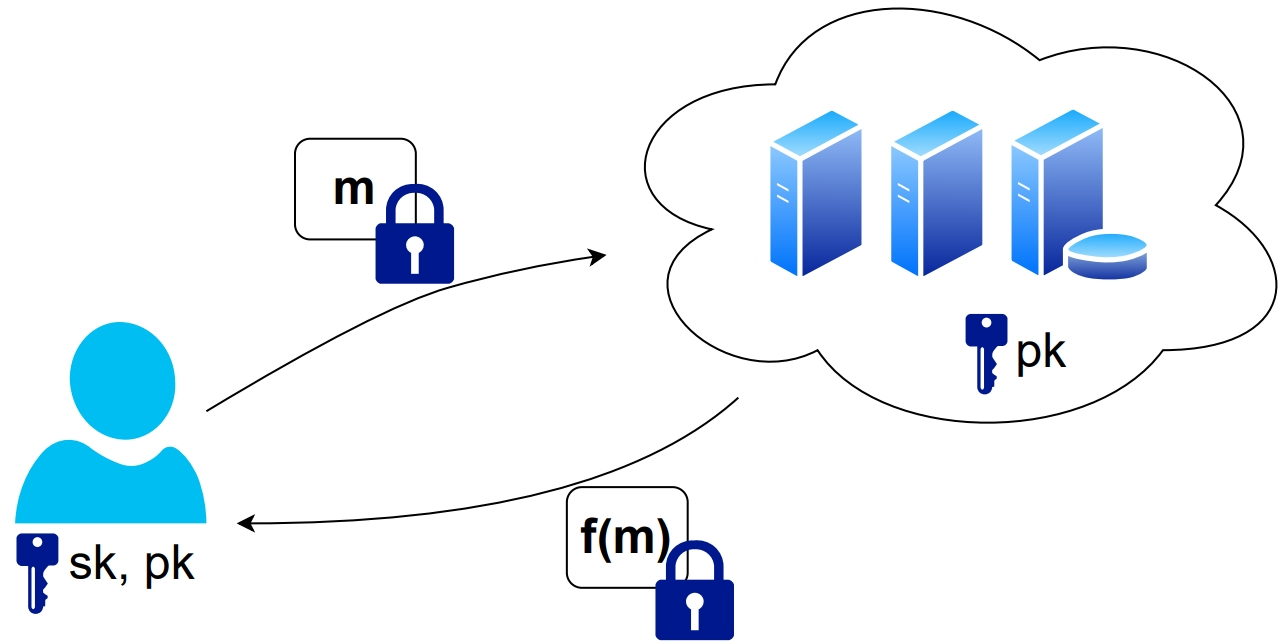
\includegraphics[scale=0.1]{fhe.jpg}
    \caption{Paper:https://ia.cr/2022/657}
\end{figure}
\end{columns}
 \vspace{-0.3cm}


Potentially very useful for cloud computing use.
 \vspace{-0.3cm}

 \pause
    \textbf{Present}: Orders of magnitude \textbf{slower} for real use.


\end{frame}

%%%%%%%%%%%%%%%%%%%%%%%%%%%%%%%%%%%%%%%%%%%%%%%%%%%%%%%%%%%%%%%%%%%%%%%%%%%%%%%%%%%%%%%%%%%%%%%%%%%%


\begin{frame}
    \frametitle{FHE}
  \begin{columns}
    \column{0.5\textwidth}
      In general, HE schemes use \texttt{Ring Learning With Errors} (RLWE) that  adds some sort of error (noise) to the encryption.

\vspace{0.3cm}
    This error grows in each operation (particularly with multiplications).

\vspace{0.3cm}
      If the error is too big the decryption will not work. or undecryptable
    \column{0.5\textwidth}
        \begin{figure}[h!]
            \centering
            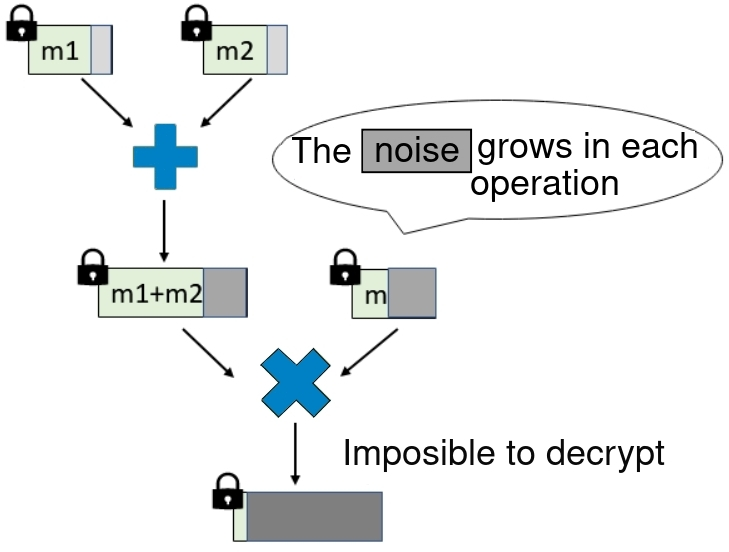
\includegraphics[scale=0.2]{multNoise.jpg}
        \end{figure}

\end{columns}    Fully Homomorphic Encryption (FHE): Unlimited number of operations. In this type of schemes
    it use \texttt{Bootstrapping} that are techniques that refresh this error.


\end{frame}
%%%%%%%%%%%%%%%%%%%%%%%%%%%%%%%%%%%%%%%%%%%%%%%%%%%%%%%%%%%%%%%%%%%%%%%%%%%%%%%%%%%%%%%%%%%%%%%%%%%%


\begin{frame}
\frametitle{Bootstrapping}

Bootstrapping vs leveling

o para la siguiente clase?
\end{frame}



%%%%%%%%%%%%%%%%%%%%%%%%%%%%%%%%%%%%%%%%%%%%%%%%%%%%%%%%%%%%%%%%%%%%%%%%%%%%%%%%%%%%%%%%%%%%%%%%%%%%


\begin{frame}
    \frametitle{Schemes}

    Many schemes. \textbf{Warning}: Many acronyms!!!

    Popular schemes by types:
    \begin{itemize}
        \item Operations on integers: BFV and BGV.
        \item Operations on real numbers: CKKS.
        \item Operations on Boolean gates: FHEW and THFHE.
    \end{itemize}


    The parameters of all schemes are application-specific and desire security.
\end{frame}

%%%%%%%%%%%%%%%%%%%%%%%%%%%%%%%%%%%%%%%%%%%%%%%%%%%%%%%%%%%%%%%%%%%%%%%%%%%%%%%%%%%%%%%%%%%%%%%%%%%%


\begin{frame}
\frametitle{Parameters - BFV, BGV, CKKS}

Most schemes works in a Polynomial Ring domain.

N will be the degree of the Polynomials (N-1).

q and t will be the mod of the coefficients.

\textbf{Ring}: a set with addition, subtraction and multiplication. (and other property's, commutative, associative, etc).

This operations of elements in a ring return elements in the ring $\rightarrow$ take modulus.




\end{frame}

%%%%%%%%%%%%%%%%%%%%%%%%%%%%%%%%%%%%%%%%%%%%%%%%%%%%%%%%%%%%%%%%%%%%%%%%%%%%%%%%%%%%%%%%%%%%%%%%%%%%


\begin{frame}
\frametitle{Math notation}
BFV, BGV and CKKS works with ciphertex  $\in \mathcal{R}_q =\mathbb{Z}_q[X]/(X^N+1)$

$\mathbb{Z}[X]$ = Set of Polynomials with integer coefficients.

$\mathbb{Z}_q[X]$ = Set of Polynomials with integer coefficients mod q.

$\mathbb{Z}_q[X]/(X^N+1)$ = The Polynomials degree N-1.


\end{frame}

%%%%%%%%%%%%%%%%%%%%%%%%%%%%%%%%%%%%%%%%%%%%%%%%%%%%%%%%%%%%%%%%%%%%%%%%%%%%%%%%%%%%%%%%%%%%%%%%%%%%


\begin{frame}
\frametitle{BFV Primitives}

    Basic Primitives (simplified):
\begin{itemize}
    \item ParamGen($\lambda$)$\rightarrow$ Params. Security $\lambda \sim$ $2^\lambda$ operation to decrypt with prob 1.
    \item KeyGen(Params) $\rightarrow$ SK, PK, EvalK
    \item Encrypt(PK, m) $\rightarrow$ c
    \item Decrypt(SK, c) $\rightarrow$ m
    \item EvalAdd(c$_1$, c$_2$) $\rightarrow$ c$_3$
    \item EvalMult(c$_1$, c$_2$) $\rightarrow$ c$_{mul}$
    \item Relinerize(c$_{mul}$, EvalK) $\rightarrow$ c$_{mul}$'
\end{itemize}

\end{frame}

%%%%%%%%%%%%%%%%%%%%%%%%%%%%%%%%%%%%%%%%%%%%%%%%%%%%%%%%%%%%%%%%%%%%%%%%%%%%%%%%%%%%%%%%%%%%%%%%%%%%


\begin{frame}
\frametitle{Workflow}

    Encryption has two phases:
\begin{itemize}
    \item From an integer m to plaintext
    \item From plain text to ciphertext c.
\end{itemize}


\begin{figure}
    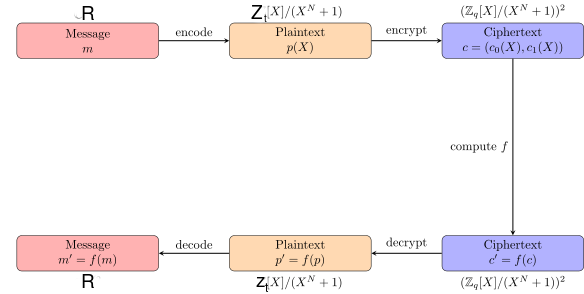
\includegraphics[width=0.85\textwidth]{bfv-diagram.png}
\end{figure}


\end{frame}


%%%%%%%%%%%%%%%%%%%%%%%%%%%%%%%%%%%%%%%%%%%%%%%%%%%%%%%%%%%%%%%%%%%%%%%%%%%%%%%%%%%%%%%%%%%%%%%%%%%%


\begin{frame}
\frametitle{BFV}

The parameters depends in the security level needed and amount of operations that will made.

% un poco mas de esto?
Bigger parameters $\approx$ Bigger ''budget error'' $\approx$ less use of Bootstrapping.

Some usual parameters to get the sense of what we are doing:

N = 8192, 16384, 32768.

q = $2^{218}$,   $2^{438}$,  $2^{881}$.

t  << q.

% que significa q/t

    \textbf{Implementations}: Residue Number System (RNS) (stay with 64bits arithmetic's), and SIMD arithmetic.
\end{frame}
%%%%%%%%%%%%%%%%%%%%%%%%%%%%%%%%%%%%%%%%%%%%%%%%%%%%%%%%%%%%%%%%%%%%%%%%%%%%%%%%%%%%%%%%%%%%%%%%%%%%


\begin{frame}
\frametitle{Encryption}

Encryption has two phases:

 - From an integer m to plaintext M $\rightarrow$ Easy, one way: binary representation as Polynomial coefficient.

    - From plaintext to ciphertext using $PK = (PK_1, PK_2)$:

\begin{itemize}
    \item Sample a polynomial $u$ from $\mathcal{R}_2$.
    \item Sample polynomial errors $e_1$ and $e_2$ form a Gaussian distribution.
    \item Calculate scaling factor $\triangle = \lfloor q/t\rfloor $
    \item Encryption of plaintext M is $C=(C_1, C_2)$
\end{itemize}
\begin{align}
    &C_1 = [PK_1 * u + e_1 + \triangle M ]_q\nonumber \\
    &C_2 = [PK_2 * u + e_2]_q\nonumber
\end{align}


\end{frame}
%%%%%%%%%%%%%%%%%%%%%%%%%%%%%%%%%%%%%%%%%%%%%%%%%%%%%%%%%%%%%%%%%%%%%%%%%%%%%%%%%%%%%%%%%%%%%%%%%%%%


\begin{frame}
\frametitle{Multiplication}

    High computational cost:
    \vspace{-0.15cm}

    $C_{mul} = C*C' = (C_1*C_1',C_1*C_2'+C_2*C_1', C_2*C_2') = (C_a,C_b,C_c)$
    \vspace{-0.15cm}

    \textbf{Problem}: If we keep multiplying, the number of Polynomials will grow and will be needed
    the squared of the SK.

    \textbf{Relinerize}:
    $EvalK = (-PK_1+SK^2, PK_2)$

    $C_{mul} = (C_a, C_b, C_c)\approx ([C_a+EvalK_1*C_c]_q, [C_b+EvalK_2*C_c]_q)$

    \textbf{Other problem}: high noise growth: we are multiplying the errors of the two ciphertexts, the result error
    grows a lot!
\vspace{-0.1cm}

    \textbf{Solution}: \vspace{-0.3cm}
    \begin{itemize} \vspace{-0.2cm}
        \item Select the lowest parameters for the ''exact'' amount  of operations needed (HE). \vspace{-0.2cm}
            \vspace{-0.25cm}
        \item Use Bootstrapping  (FHE). Even more demanding (multiple multiplications like $C_{mul}$).
    \end{itemize}
\end{frame}
%%%%%%%%%%%%%%%%%%%%%%%%%%%%%%%%%%%%%%%%%%%%%%%%%%%%%%%%%%%%%%%%%%%%%%%%%%%%%%%%%%%%%%%%%%%%%%%%%%%%

\begin{frame}
\frametitle{Recap}

    \textbf{Rembember!} All things are high degree polynomials with huge coefficient.

For a single multiplication of two numbers:
\begin{itemize}
    \item Enconde and encrypt: Sample the errors and parts of the Keys and multiply them to generate the Keys.
    \item Multiplication: Multiply the different parts of the ciphertexts.
    \item Relinerize: Multiply the result with the evaluation key.
\end{itemize}

Each homomorphic operation is $10^3 \sim 10^6$ times slower than unencrypted.
\pause

Large footprint in memory.
An encrypted date can occupy $10^5$ more space.

\pause
The schemes are iterative, operating many time with each data.
\pause



\end{frame}
%%%%%%%%%%%%%%%%%%%%%%%%%%%%%%%%%%%%%%%%%%%%%%%%%%%%%%%%%%%%%%%%%%%%%%%%%%%%%%%%%%%%%%%%%%%%%%%%%%%%


\begin{frame}
\frametitle{Research}

    The usual way of approaching this problem of speed (and others):  accelerating the server
    part.
\begin{itemize}
   \item Accelerating the polynomial multiplication:
    For these they use Number Theoretic Transform (NTT), a Discrete Fourier Transform (DFT) over a ring.
    \item New schemes.
    \item New upgrades in the schemes (like RNS).
   \item New methods of Bootstrapping.
   \item Software Optimization.
   \item Hardware Acceleration (GPUs, FPGA, specific designs).
\end{itemize}

\end{frame}
%%%%%%%%%%%%%%%%%%%%%%%%%%%%%%%%%%%%%%%%%%%%%%%%%%%%%%%%%%%%%%%%%%%%%%%%%%%%%%%%%%%%%%%%%%%%%%%%%%%%


\begin{frame}
\frametitle{New approach}


    The new approach:  accelerate the client side.

    CHACO: \textbf{C}lient-aided \textbf{H}E for \textbf{O}paque \textbf{C}ompute \textbf{O}ffloading.


    Is a client-aided HE: operate by using the client multiple times.

    Prior systems of these type also focus on accelerating the server part.

    % para que y cuando se utiliza el rotacional redundancy
    \begin{itemize}
        \item Reduces ciphertext size $\rightarrow$ reducing cominication.
        \item New algorithm: rotational redundancy $\rightarrow$ reduces computation costs.
        \item Reduction of parameters values $\rightarrow$ reduces computation costs.
        \item Minimice client costs.
        \item Hardware acceleration for client: CHACO-TACO.
    \end{itemize}


\end{frame}

%%%%%%%%%%%%%%%%%%%%%%%%%%%%%%%%%%%%%%%%%%%%%%%%%%%%%%%%%%%%%%%%%%%%%%%%%%%%%%%%%%%%%%%%%%%%%%%%%%%%

\begin{frame}
\frametitle{}
The paper poitns to use for DNNs, PAgeRank, KNN and K-means.

ML modeol ->inference as a service
data privacy -> offloading exposes sensitive user data to a shared potentially untrasted offload server.

HE problemns: only polynomial calculation, non linearity si imposible, only approximate. client-aided solve this.

many mpc proposals use the client solving this problem but are ineficient because de client is slow.
    Large ciphertext comunication

    chaco is a mpc that minimiza the client cost. Order of magnitude less that others

    encrypted linear operations on the server.
    plaintext non linear operations on the client.


\end{frame}

%%%%%%%%%%%%%%%%%%%%%%%%%%%%%%%%%%%%%%%%%%%%%%%%%%%%%%%%%%%%%%%%%%%%%%%%%%%%%%%%%%%%%%%%%%%%%%%%%%%%


\begin{frame}
\frametitle{}

now Encrpytion and decryption, that before was one time per  computation, now is use many times beeing now a bottleneck.

CHACO-TACO eliminates this.

chaco for bfv and ckks.

DONDE hace rotational en BFV? y para que sirve.

ACA REPITO, VER ARRIBA COMO PONERLO.
    \begin{itemize}
        \item CHACO, a Client-optimized system for privacy-preserving computation enabiling encrpyted computing for resorucescontraied devices.
        \item Rotational redundancy.
        \item CHACO-taco
        \item collection fo chaco based encrypted worloads.
    \end{itemize}

\end{frame}
%%%%%%%%%%%%%%%%%%%%%%%%%%%%%%%%%%%%%%%%%%%%%%%%%%%%%%%%%%%%%%%%%%%%%%%%%%%%%%%%%%%%%%%%%%%%%%%%%%%%


\begin{frame}
\frametitle{}
complejidad

aproximate non linear functions acumulate noise quickly and require large HE parameters. large ciphertext, harder to comunicate and compute.
\end{frame}


%%%%%%%%%%%%%%%%%%%%%%%%%%%%%%%%%%%%%%%%%%%%%%%%%%%%%%%%%%%%%%%%%%%%%%%%%%%%%%%%%%%%%%%%%%%%%%%%%%%%


\begin{frame}
\frametitle{}

\end{frame}


%%%%%%%%%%%%%%%%%%%%%%%%%%%%%%%%%%%%%%%%%%%%%%%%%%%%%%%%%%%%%%%%%%%%%%%%%%%%%%%%%%%%%%%%%%%%%%%%%%%%


\begin{frame}
\frametitle{}

\end{frame}
%%%%%%%%%%%%%%%%%%%%%%%%%%%%%%%%%%%%%%%%%%%%%%%%%%%%%%%%%%%%%%%%%%%%%%%%%%%%%%%%%%%%%%%%%%%%%%%%%%%%


\begin{frame}
\frametitle{}

\end{frame}


%%%%%%%%%%%%%%%%%%%%%%%%%%%%%%%%%%%%%%%%%%%%%%%%%%%%%%%%%%%%%%%%%%%%%%%%%%%%%%%%%%%%%%%%%%%%%%%%%%%%


\begin{frame}
\frametitle{}
\Huge

\begin{center}
   Questions?
\end{center}
\end{frame}


%%%%%%%%%%%%%%%%%%%%%%%%%%%%%%%%%%%%%%%%%%%%%%%%%%%%%%%%%%%%%%%%%%%%%%%%%%%%%%%%%%%%%%%%%%%%%%%%%%%%


\end{document}

